% catch up the thread from the introduction why user data is important
Careful analysis on Big Data can enhance business domain understanding for any company. Accordingly, Big Data has became a widely studied and interesting topic all around the field Information Technology in the recent years, both in scientific and industrial research \cite{inmon2007tapping, introtodatamining}. Significant amount of the data is somehow related to the users of the software at hand. Such data often incorporates essential data about the users themselves, such as their demographic data, preferences or how they interact with the software 
\cite{jang2015noreciprocity, hu2014we, jang2016teensengagemorewithfewerphotos, han2016teensarefrommars, socialdiversityongithub}.

% what is user behavior?
% Despite the fact the term user behavior is widely studied, researchers claim that its concept is used rather ambiguously \cite{waheed2017investigation}. According to Waheed et al., many studies in the field of social media sites address topics such as gender, age and cultural differences, self–representation or privacy concerns, which are all related to user behavior \cite{waheed2017investigation}. These aspects are studied typically in order to enhance the service package of the social media site of discussion 

% why should user data be defined?
While exploring the background and related literature of this study it was identified, that the concept of user data is not commonly used among researchers. Most of the reviewed studies simply use the terminology that is related to the domain of the study, for instance like activities, user reviews or ratings. The studies often utilize demographic data (typically gender and age), the two concepts are often used separately. 

% what is user data? what does it include or exclude?
To set a common ground and understanding for the rest of this thesis work, the concept of user data is defined. User data in this study covers two major kind of data that is related to users. On one hand it covers data, which is willingly uploaded and generated by users. On the other hand, user data consists of data which generated through interactions while using software solutions (typically online). User data in this study is the combination of these two aspects, which is demonstrated on Figure \ref{user_data_venn}.

% demographic characteristics
The first part of user data typically consists of the demographic characteristics of the users and the content which they have generated \cite{han2016teensarefrommars}. Traditionally demographic data is often collected via surveys and questionnaires by researchers. This kind of data often can be found on social media profiles where social demographic information, such as gender, age and nationality are shared. As a result, this kind of data can be obtained relatively easily in vast amount, if users as eager to share with the software service provider.

% digital footprints
Secondly, data gathered during the usage of a software is an important source of information for scientific studies. Researchers use the term digital footprint \cite{youyou2015computer} to describe this kind of data, which composes the second type of user data in this research. Such digital footprints can vary a lot depending on the software of discussion, but typically consists of like activities, user comments, photos, posts on social media, ratings in movie databases or browsing history. 

\begin{figure}[h] 
  \begin{center}
    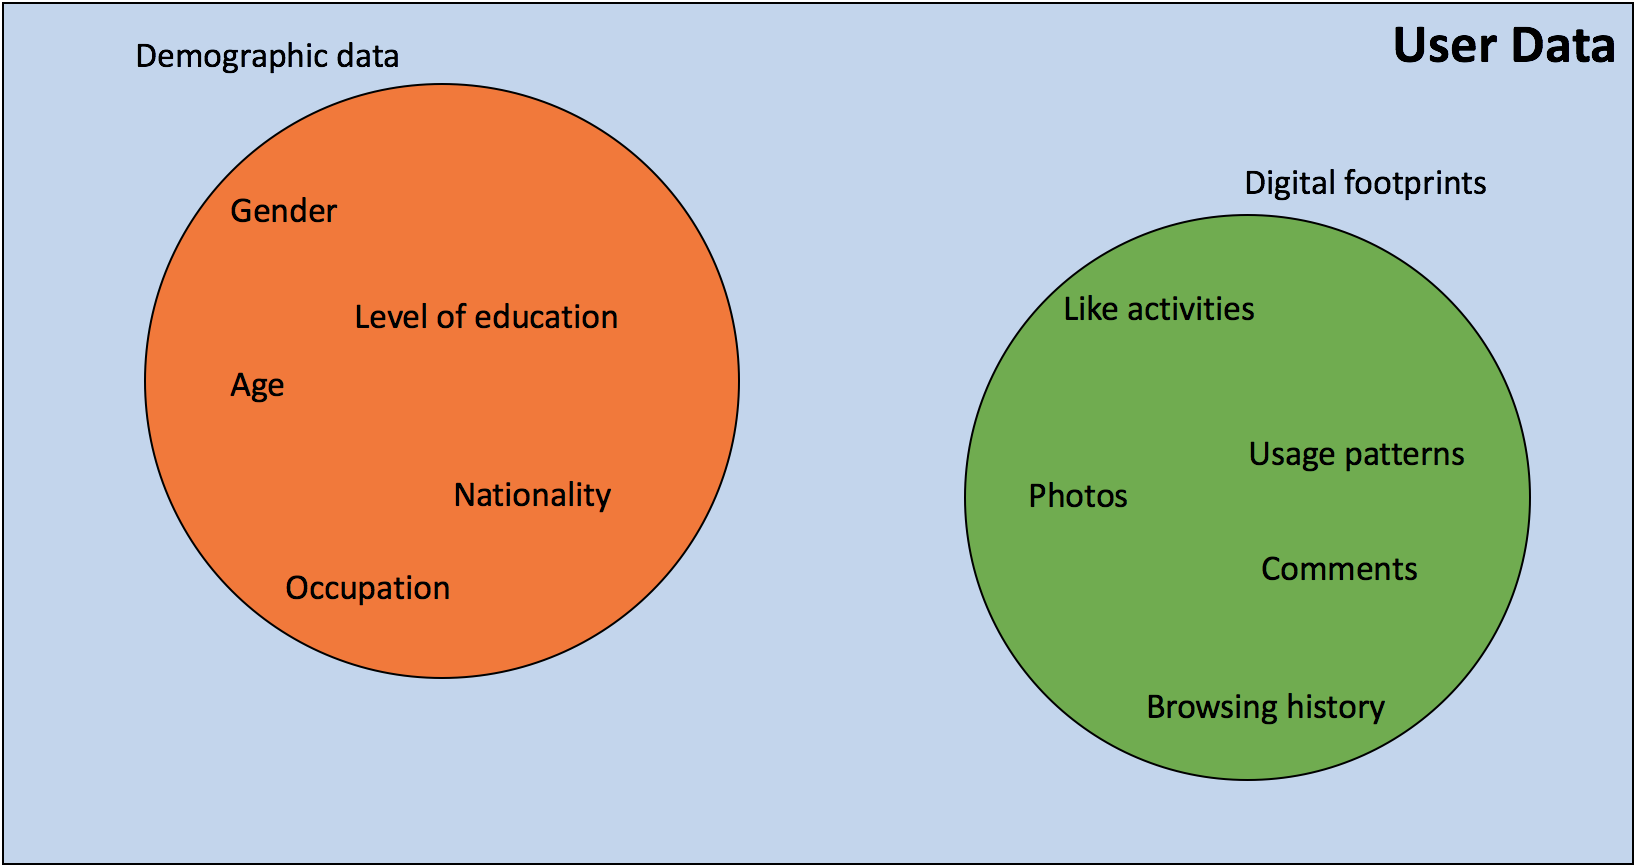
\includegraphics[width=3in]{Images/user_data_venn.png}
    \caption{User data in this research is the combination of users' demographical characteristics and digital footprints (the data items mentioned are only examples, there could be other data items in both sets).}
    \label{user_data_venn}
  \end{center}
\end{figure}

\subsection{Related research}
Previous research have proven the relevance and applicability of Data Mining methods on user data with various goals. These goals include, but are not limited to studying like activities \cite{jang2015noreciprocity, jang2016teensengagemorewithfewerphotos, ottoni2013ladies, guy2016whatsyourorganizationlike, jang2015no}, user comments \cite{jang2016teensengagemorewithfewerphotos}, tags under images \cite{jang2016teensengagemorewithfewerphotos}, image content \cite{hu2014we, bakhshi2014faces}, movie ratings \cite{saraee2004data, kabinsingha2012movie} and web usage mining \cite{webusagemining}. All of these studies have revealed interesting findings in their domain based on the data at hand. Moreover, as service providers often get access to user demographics-related data through social network sites in the present time, new possibilities become available to seek correlation between user segments. The paragraphs to follow explain some of the use cases where user data was utilized in order to adress RQ1 of this study.

% explain that these are often not studied together but rather separately 
The concepts of demographical characteristics and digital footprints are widely studied in the research field, but often only separately, focused on one certain area. Demographic characteristics play a role in analyzing user adoption and behavior, for instance in the banking industry. The study conducted by Wang and Petrounias \cite{chinesemobilebankingusers} shows that mobile banking in China is more popular among middle-aged males, while the younger generation has not adopted to the new trends yet. By utilizing Big Data analytics, the group of citizens and products for the upcoming marketing campaigns were revealed \cite{chinesemobilebankingusers}, which greatly enhances the marketing activities of financial organizations. Social diversity was also studied by other researchers in the context of software development growth \cite{socialdiversityongithub}. In their study, Au\'e et al. \cite{socialdiversityongithub} have clearly identified correlation between the success of open source projects and the contributors' gender and cultural diversity by utilizing well chosen statistical methods.

% what kind of results were derived in the past from end-user data analysis? 
Movie databases often contain user reviews on movies, actors and producers of all sort. Such databases are open and are available for the public, and therefore the amount of data has grown huge over the past years. Unsurprisingly, databases like the Internet Movie Database (IMDB) has drawn the interest of researchers \cite{saraee2004data, kabinsingha2012movie, sumathi2013performance}. The successful application of statistical methods and data mining techniques have revealed interesting findings. Studies have proven that larger budget for movies does not necessarily result in good ratings by the public, while actors have higher impact on the opinion of the audience \cite{saraee2004data}. On top of deriving such conclusions, machine learning techniques are emerging to predict future movie rating data, based on prior reviews of users \cite{saraee2004data} or the analysis of genre and other attributes of movies \cite{kabinsingha2012movie}. Opinion mining is another area of development in this field \cite{sumathi2013performance}, however it is mainly operating on unstructured, textual data via the reviews of movies. 

% how do researches on social media website data see the user data analysis?  
Social Networking Sites (SNSs) are another trending source in discovering the secrets of user data as the number of scientific publications in the topic has increased significantly in the recent years \cite{waheed2017investigation}. Various researches have applied advanced Data Mining techniques on Instagram data \cite{jang2015noreciprocity, bakhshi2014faces, hu2014we, jang2016teensengagemorewithfewerphotos, han2016teensarefrommars}, more specifically on the tags and comments that are attached to the images. Similarly, like activities and user-generated content is studied by the scientists. It was revealed, that Instagram users can be divided into two groups based on their activities: specialists, who publish and seek content around a certain topic of interest; and generalists, who are interested in all kinds of genres in the social media site \cite{jang2015noreciprocity}. Data Mining techniques also allowed researchers to conclude, that the teenager users of Instagram tend to be more active, faster to react and more open to communicate with other users on social media \cite{jang2016teensengagemorewithfewerphotos, han2016teensarefrommars}. Furthermore, it was discovered that media content with human faces are more engaging than other type of media \cite{bakhshi2014faces}. Finally, rich social media data allowed researchers to analyze behavior and user preferences among genders, age groups and locations \cite{farseev2015harvestingmultiplesources}.

Like activities performed on social media are widely studied concept \cite{bakhshi2014faces, jang2015noreciprocity, jang2016teensengagemorewithfewerphotos, ottoni2013ladies}. Comments, hashtags and content that is generated by users are also widely studied \cite{bakhshi2014faces, jang2016teensengagemorewithfewerphotos, hu2014we, bakhshi2014faces} and also contribute to this kind of data in this study. However, little research has been conducted in the field on how these usage patterns can be projected onto demographical data, which can greatly contribute to understand user behavior of certain target groups. 

% where is all this research coming from?
Interestingly, most of the SNS-related studies are conducted in the United States of America and Asia \cite{waheed2017investigation}. According to Waheed, Anjum and Khawaja, only a few studies were conducted in the European region, which allows to conclude that there is a room for research in the area \cite{waheed2017investigation}. However, it is important to highlight, that due to the wide popularity of the international social networks (such as Facebook, Instagram or Pintrest), some part of the data may be derived from users in the European continent. They have also pointed out that some researches focus on sites, that are specific to a particular region or country \cite{waheed2017investigation}, which means the findings are strongly related to the cultural environment of the user base. Nevertheless, this finding may imply either the lack of interest in the area or the variance in cultural background of users. 

% facebook reactions
Recently Facebook has introduced reactions among their features. Through reactions, users can not only "like" content, but also express other emotions, such as love, joy, amazement, anger or sadness \cite{shouldfacebookusereactions, howarenewspublishersreactingonfacebook}. This way users' emotional feelings about the content can be collected easily and efficiently. Shortly after its release, it was identified that the new feature is very popular and generally engages a wider audience than previous likes and comments \cite{shouldfacebookusereactions}. Study also shows, that reactions are a great way for publishers to get a feedback on the public's opinion \cite{howarenewspublishersreactingonfacebook}. On top of that, reactions offer an easy way for content providers to organize a by assigning one of the available reactions to the participants and asking the users to react on the content with their favorite's reaction \cite{shouldfacebookusereactions}. The limitation on such polls is that users have the possibility to choose only one of the reactions and hence only one of the participants as their answer to the voting. Despite its wide availability and potential, there was no comprehensive study conducted in this area until this date.

% what does user data analysis reveal in a corporate social media environment? [refer to \cite{guy2016whatsyourorganizationlike}]
Social media platforms in enterprise environment are studied similarly to regular social networks \cite{guy2016whatsyourorganizationlike}. Despite the fact that the two types of social media platforms share many features, analysis performed in enterprise environment can provide great insights about how employees interact and cooperate. Among many other findings, studies have shown that blogs posts in an enterprise social media site tend to be more engaging and contribute to form communities inside the organization \cite{guy2016whatsyourorganizationlike}. Such insights are essential for higher management, because it can be used for instance to identify departments that tend to be less interactive or engaged.  

\subsection{Tools and methods}
Various methods were utilized in previous research to conclude the findings above. The major categories of the techniques and their purposes are explained in the paragraphs to follow. Table \ref{table_of_techniques} below lists the same findings.

% what methods are utilized? 
  % multiple data sources
  The combination of multiple data sources containing users' demographic data, such as Facebook, Instagram, Pintrest or other social media services, is a common practice in researches \cite{farseev2015harvestingmultiplesources, ottoni2013ladies}. Researchers have managed to perform complete demographic profiling and concluded that the integration of multiple data sources is indeed a great method of enhancing performance on user data analysis \cite{farseev2015harvestingmultiplesources}. 
  
  Utilizing additional tools, existing datasets can be further enhanced for data analysis purposes. A great specimen for this is computer vision, which is used in numerous studies to identify content of photos \cite{hu2014we, farseev2015harvestingmultiplesources}. In two of the reviewed papers \cite{han2016teensarefrommars, bakhshi2014faces}, computer vision techniques are utilized to identify faces on and predict ages of people from photos uploaded to social media sites. Through these researches, computer vision was proven to be a powerful tool to facilitate the knowledge by providing researchers further data for their studies. 

  % text processing techniques
  Text processing techniques are potentially the most common way to discover the insights of user data. The Linguistic Inquiry and Word Count (LIWC) and Latent Dirichlet Allocation (LDA) methods are used by researchers \cite{ottoni2013ladies, farseev2015harvestingmultiplesources, jang2016teensengagemorewithfewerphotos} for extracting linguistic features of text. In their study, Jang et al. use this technique to identify keywords and perform topic modelling based on users' comments and hashtags on Instagram \cite{jang2016teensengagemorewithfewerphotos}. Topic modelling was also applied for analyzing genres of movies by their title and description \cite{kabinsingha2012movie}. Applying natural language processing techniques also allowed researchers to infer age and gender of users \cite{han2016teensarefrommars} who have commented on content on Instagram. Utilizing these methods greatly contribute to the understanding of data gathered, which can lead to richer analysis and pattern recognition on the dataset at hand. 

  % supervised ML techniques
  Supervised machine learning appears to be a popular technique for prediction tasks performed on user data. For example, decision trees are utilized as prediction tools for the purposes of identifying audience of mobile banking software in China \cite{chinesemobilebankingusers}. Decision trees were also successfully used for movie rating prediction \cite{saraee2004data} and classification of movies \cite{kabinsingha2012movie}. Bayesian networks in the same study \cite{kabinsingha2012movie} are also investigated and are found as the most suitable method for predictions in the field of movie rating prediction. Ensemble Modeling, which is another supervised learning method, is successfully used for user profile learning on social media sites \cite{farseev2015harvestingmultiplesources}. Similarly, Support Vector Machines and Logistic Regression was utilized for predicting age group of users based on their social media activities \cite{han2016teensarefrommars}. Last, but not least Negative Binomial Regression is put in use to model like activities in researches \cite{jang2015no, bakhshi2014faces}.

  % unsupervised learning - less popular but still possible
  Unsupervised machine learning techniques are also present in the literature, however on a smaller scale. As an example, clustering is used by Saraee White and Eccleston \cite{saraee2004data} for detecting relationships between the ratings given on a movie and the year it was published. The study by Hu et al. \cite{hu2014we} uses the k-means algorithm was used successfully to create five clusters of Instagram users based on the type of content they have uploaded to Instagram. These results share similarities with another study by Jang et al. \cite{jang2015no}, where generalist and specialist groups were identified based on their like activities based on natural language processing techniques. 

  % frequent itemset
  Frequent Itemset Analysis is utilized by Ottoni et al. \cite{ottoni2013ladies} for user portfolio analysis and detecting differences among genders in their data. By utilizing this technique, the researchers have identified significant differences between the two genders' preferences in terms of online content \cite{ottoni2013ladies}. Based on their research it can be concluded, that this technique can be a great tool to perform comparative analyses between demographic groups or pieces of content. 

  \begin{table}[!t]
    \renewcommand{\arraystretch}{1.5}
    \caption{The summary of utilized data mining techniques on user data in other researches.}
    \label{table_of_techniques}
    \centering
      \begin{tabular}{c||c}
        Technique & Number of studies \\ 
        \hline
        Computer vision & 3  \\
        Text/Natural language processing & 5 \\
        Unsupervised machine learning & 2 \\
        Supervised machine learning & 5 \\
        Frequent Itemset Analysis & 1
      \end{tabular}
  \end{table}

\subsection{Discussion/summary}
% variance in user data (especially in the digital footprints)
The results of this literature review shows, that there is not a common understanding on the term of user data among researchers. While demographic data is very well understood, digital footprints (data gathered during the usage of a software) are less commonly studied for research purposes. In other words, user demographic data and digital footprints are not usually brought under the same hood, are often vaguely defined and sometimes are studied separately. It is clearly identified that the careful utilization of user demographic and digital footprints, software service providers and researchers can retrieve previously unknown information about users' behavioral characteristics. 

Access to demographic data in the present time seems to be getting easier for researchers. Social networks already have standard ways of helping users to authenticate themselves while using other services (in other words use their social network credentials to use other services), businesses can get access to rich demographic data of their user base easily. 

% why are these researches interesting? What do we learn from the society by performing analysis on user data? 
The examples in the previous sections demonstrate the relevance of Data Mining and Machine Learning methods in the field of user data analysis. The proper application these methods allow us to learn more about the society as well as human behavior, which was not possible in the past. This information is essential for business operations, because it gives insights on the user groups, their preferences and what kind of content keeps the audience engaged. Furthermore, these tools provide researchers novel ways to look at human behavior and differences between demographic groups.

From the chosen set of related studies it seems, that natural language processing and supervised machine learning techniques are the most common approaches for conducting research on user data. The encouraging results achieved by other researchers prove the relevance of computational techniques applied on user data in a wide range of development areas, such as banking, social media, online movie databases, user portfolio analysis to name a few. Despite not being part of this short study, recommender systems could be an interesting topic of further development and discussion in the area.

In the past these kind of insights were unavailable to researchers and content providers. In the present time, access to this information can facilitate research, business processes, helps determining the future content, analyzing trends and understanding target groups of particular services better. In sum, modern data mining techniques created the potential to study human preferences and behavior from a different, novel angle.

% how does all of this relate to the rest of this research? 